\chapter{Implementacja systemu kategoryzacji}
\label{cha:implementacja}

System kategoryzacji jest kompletną aplikacją, która oferuje gromadzenie danych, przetwarzanie ich, wyliczanie rezultatów, a także interakcję z użytkownikiem. Modelowo taki system powinien zawierać trzy elementy:
\begin{enumerate}
    \item Warstwa persystencji danych.
    
    Element systemu, który ma za zadanie trwałe przechowywanie danych. Zwykle jego rolę pełni baza relacyjna. Możliwe jest jednak wykorzystanie innych systemów takich jak bazy nierelacyjne (NoSQL). Głównym założeniem tego elementu jest zachowywanie stanu aplikacji nawet jeśli zostanie ona zamknięta.
    
    \item Warstwa logiki aplikacji.
    
    Część odpowiadająca za przetwarzanie zapytań użytkownika, komunikację z bazą danych oraz przetwarzanie danych. Zazwyczaj modeluje ona pewne procesy biznesowe.
    
    \item Warstwa prezentacji.
    
    Element odpowiedzialny bezpośrednio za interakcję z użytkownikiem. Przekazuje on żądania użytkownika do warstwy logiki aplikacji oraz prezentuje odpowiedzi w czytelnej dla człowieka formie. Pełni ona bardzo ważną rolę w kwestii odbioru aplikacji przez użytkownika.
\end{enumerate}

\section{Warstwa persystencji danych}

Jako warstwę przechowywującą dane aplikacji użyłem produktu firmy Amazon - DynamoDB. Jest to baza nierelacyjna charakteryzująca się niskim kosztem zapisu i odczytu danych. Została ona obszernie opisana w rozdziale \ref{cha:wprowadzenieTechnologiczne}.

W procesie implementacji aplikacji używałem DynamoDB w dwóch formach:

\begin{enumerate}
    \item Zdalnie poprzez platformę Amazon Web Service.
    
    AWS jest jedynym miejscem w którym mamy możliwość ustawienia DynamoDB w wersji produkcyjnej. Najważniejszym parametrem jej konfiguracji jest region, czy miejsce gdzie nasza baza będzie się fizycznie znajdowała. Najkorzystniejszym wyborem jest ten sam region w którym działa aplikacja - wtedy opóźnienie w przesyłaniu danych będzie najmniejsze.
    
    \item Na lokalnym środowisku.
    
    Amazon udostępnia nam trzy sposoby na uruchomienie DynamoDB na środowisku lokalnym:
    
    \begin{enumerate}
        \item Poprzez plik .jar
        \item Używając narzędzia budowania aplikacji - Apache Maven
        \item Poprzez obraz Dockera
    \end{enumerate}
    
    Z powodu dobrej znajomości Dockera zdecydowałem się na trzeci sposób. Obraz znajduje się w oficjalnym rejestrze \footnote{https://hub.docker.com/r/amazon/dynamodb-local/} i jesteśmy w stanie go pobrać i uruchomić przy użyciu jednej komendy (pod warunkiem, że mamy zainstalowanego Dockera):
    
    \begin{verbatim}
        docker run -p 8000:8000 amazon/dynamodb-local
    \end{verbatim}
    
    Po wykonaniu tej operacji lokalna instancja DynamoDB jest dostępna na porcie 8000. Z tak skonfigurowanym środowiskiem jesteśmy w stanie komunikować się na dwa sposoby:
    
    \begin{enumerate}
        \item AWS CLI
        
        Jest to narzędzie konsolowe do obsługi usług AWS. Z jego pomocą jesteśmy w stanie tworzyć oraz zarządzać serwisami umieszczonymi w chmurze Amazona. W DymanoDB nową tabelę możemy stworzyć za pomocą komendy:
        
        \begin{verbatim}
aws dynamodb create-table \
    --table-name User \
    --attribute-definitions \
        AttributeName=Id,AttributeType=S \
        AttributeName=Name,AttributeType=S \
    --key-schema 
        AttributeName=Id,KeyType=HASH \
        AttributeName=Name,KeyType=RANGE \
    --provisioned-throughput ReadCapacityUnits=1,WriteCapacityUnits=1
    --endpoint-url http://192.168.99.100:8000
        \end{verbatim}
        
        Należy zauważyć, że parametr endpoint-url wskazuje na lokalną instancję DynamoDB uruchomioną w kontenerze Dockera. Gdyby nie został on podany wtedy AWS CLI wymaga uwierzytelnienia się w usłudze AWS i próbowałby utworzyć zasoby w chmurze.
        
        \item AWS SDK
        
        Amazon zapewnia nam obszerne SDK do wielu języków programowania. Pozwala to na wygodną integrację z usługami AWS z tworzonymi aplikacjami. W systemie tworzonym w ramach tej pracy korzystałem z języka Python, do którego AWS SDK znajduje się w ramach pakietu boto3. Przykład tworzenia analogicznej tabeli poprzez AWS SDK:
        
        \begin{verbatim}
boto3.resource('dynamodb', endpoint_url='http://localhost:8000')\
.create_table(
    TableName='Users',
    KeySchema=[
        {
            'AttributeName': 'label',
            'KeyType': 'HASH'
        },
        {
            'AttributeName': 'content',
            'KeyType': 'RANGE'
        }
    ],
    AttributeDefinitions=[
        {
            'AttributeName': 'label',
            'AttributeType': 'S'
        },
        {
            'AttributeName': 'content',
            'AttributeType': 'S'
        }
    ],
    ProvisionedThroughput={
        'ReadCapacityUnits': 1,
        'WriteCapacityUnits': 1
    }
)
        \end{verbatim}
    \end{enumerate}
    
\end{enumerate}

\subsection{Struktura danych}

Charakterystyka rozproszonych nierelacyjnych baz danych wymaga od programisty specjalnego podejścia do projektowania struktury w jakiej dane będą przechowywane. W bazach relacyjnych dąży się do jak najlepszej normalizacji i braku duplikacji. Podczas, gdy używamy DynamoDB każda tabela może być rozproszona na wiele partycji, przez co ilość danych nie stanowi ograniczenia. Również koszt ich przechowywania jest niski, przez co warto duplikować dane, jeśli może to mieć wpływ na szybkość działania systemu.

W podstawowym modelu danych przechowywanych w ramach systemu klasyfikacji skupiłem się na prostej strukturze zwierającej trzy atrybuty:

\begin{enumerate}
    \item Label - kategoria która opisuje daną próbkę
    
    \item Source - źródło z którego próbka pochodzi
    
    \item Content - zawartość próbki
\end{enumerate}

Projektowanie tabel w DynamoDB najlepiej zacząć od ustalenia jakie kwerendy będziemy chcieli na nich wykonywać. W przypadku powyższych danych ustaliłem dwie opcje:

\begin{enumerate}
    \item Pobieranie danych według atrybutu 'Label'
    
    \item Pobieranie danych według atrybutu 'Source'
\end{enumerate}

Dodatkowym założeniem, które przyjąłem był brak duplikatów w poszczególnych tabelach. Uczenie algorytmów zduplikowanymi próbkami zaburzałoby cały proces i mogło by prowadzić do błędnych wyników. Z tego powodu zdecydowałem się zapewnić unikalność danych na poziomie warstwy persystencji danych.

Biorąc pod uwagę powyższe wymagania zdecydowałem się na poniższy schemat:

\begin{figure}[H]
    \centering
    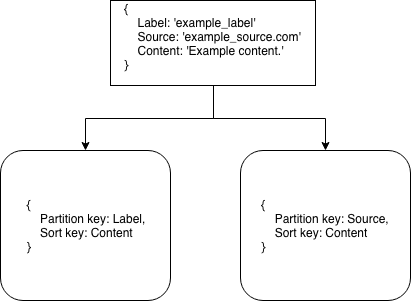
\includegraphics[width=10cm]{data_structure.png}
    \caption{Struktura danych}
\end{figure}

Pierwszą ważną cechą jest zduplikowanie danych w dwóch tabelach - na każdej bedzie wykonywana inna kwerenda. Tabela 'content\_by\_label' posłuży do odczytania danych po atrybucie 'Label', natomiast gdy chcemy pobrać wszystkie dane pochodzące z jednego źródła, wtedy użyjemy tabeli 'content\_by\_source'.

Unikalność danych zapewniło nam użycie Primary Key z dwoma atrybutami. Primary Key składa się z dwóch części:

- Partition key - atrybut, którego hash określi na której partycji znajdzie się dany rekord

- Sort key - atrybut według którego dane będą posortowane w obrebie partycji

Primary key musi być zawsze unikalny. Z tego powodu zastosowanie par ('Label', 'Content') oraz ('Source', 'Content') pozwoliło mi zapewnić unikalność danych w obrębie każdej z tabel.

\begin{figure}[H]
    \centering
    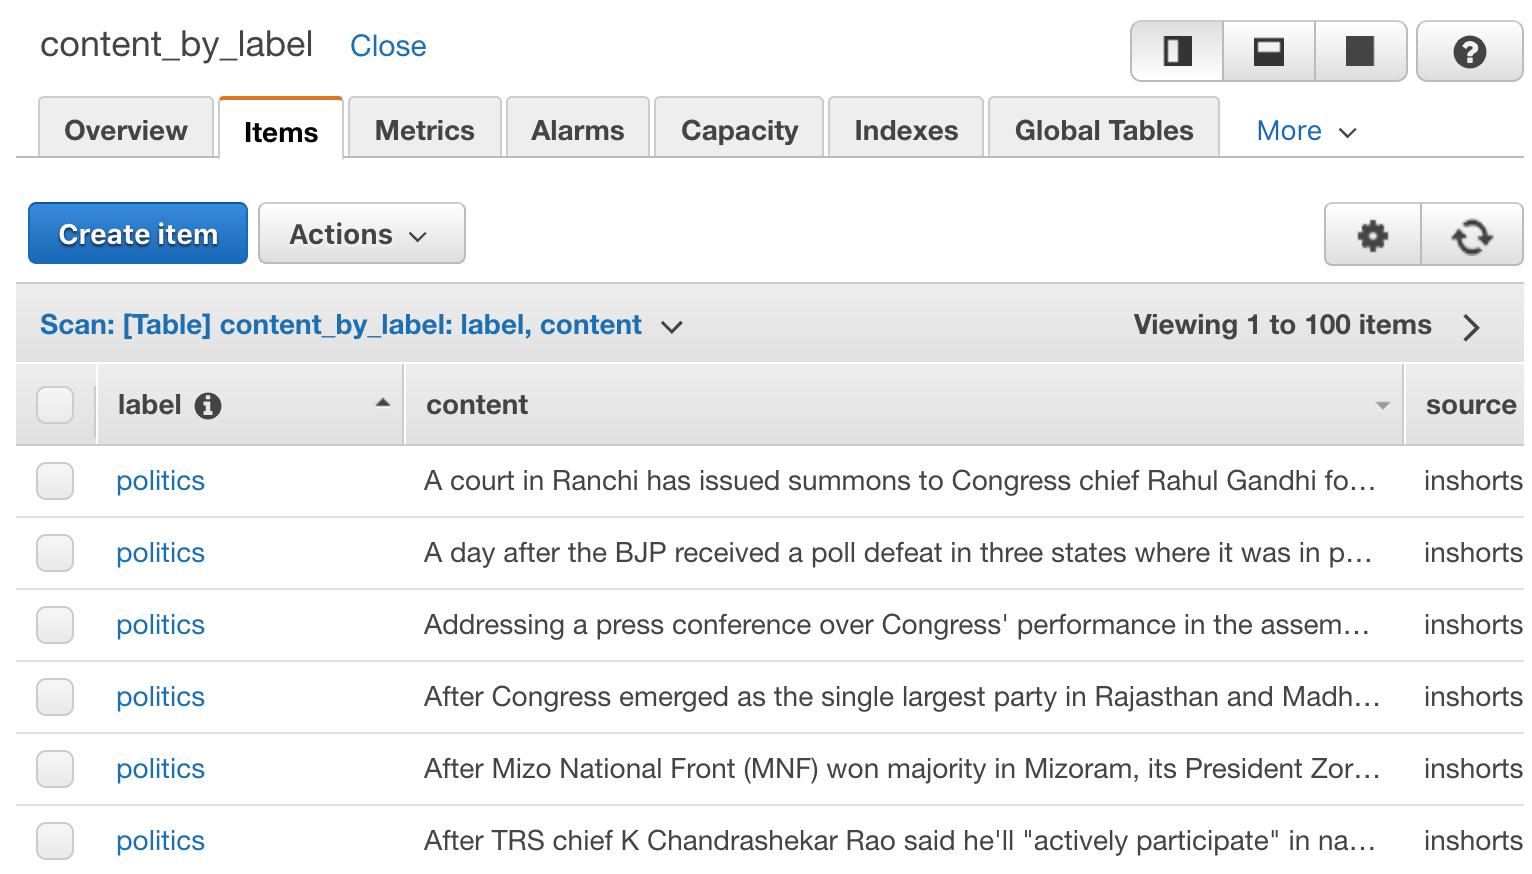
\includegraphics[width=10cm]{dynamo_by_label.png}
    \caption{Fragment tabeli content\_by\_label widocznej z poziomu konsoli AWS}
\end{figure}

\begin{figure}[H]
    \centering
    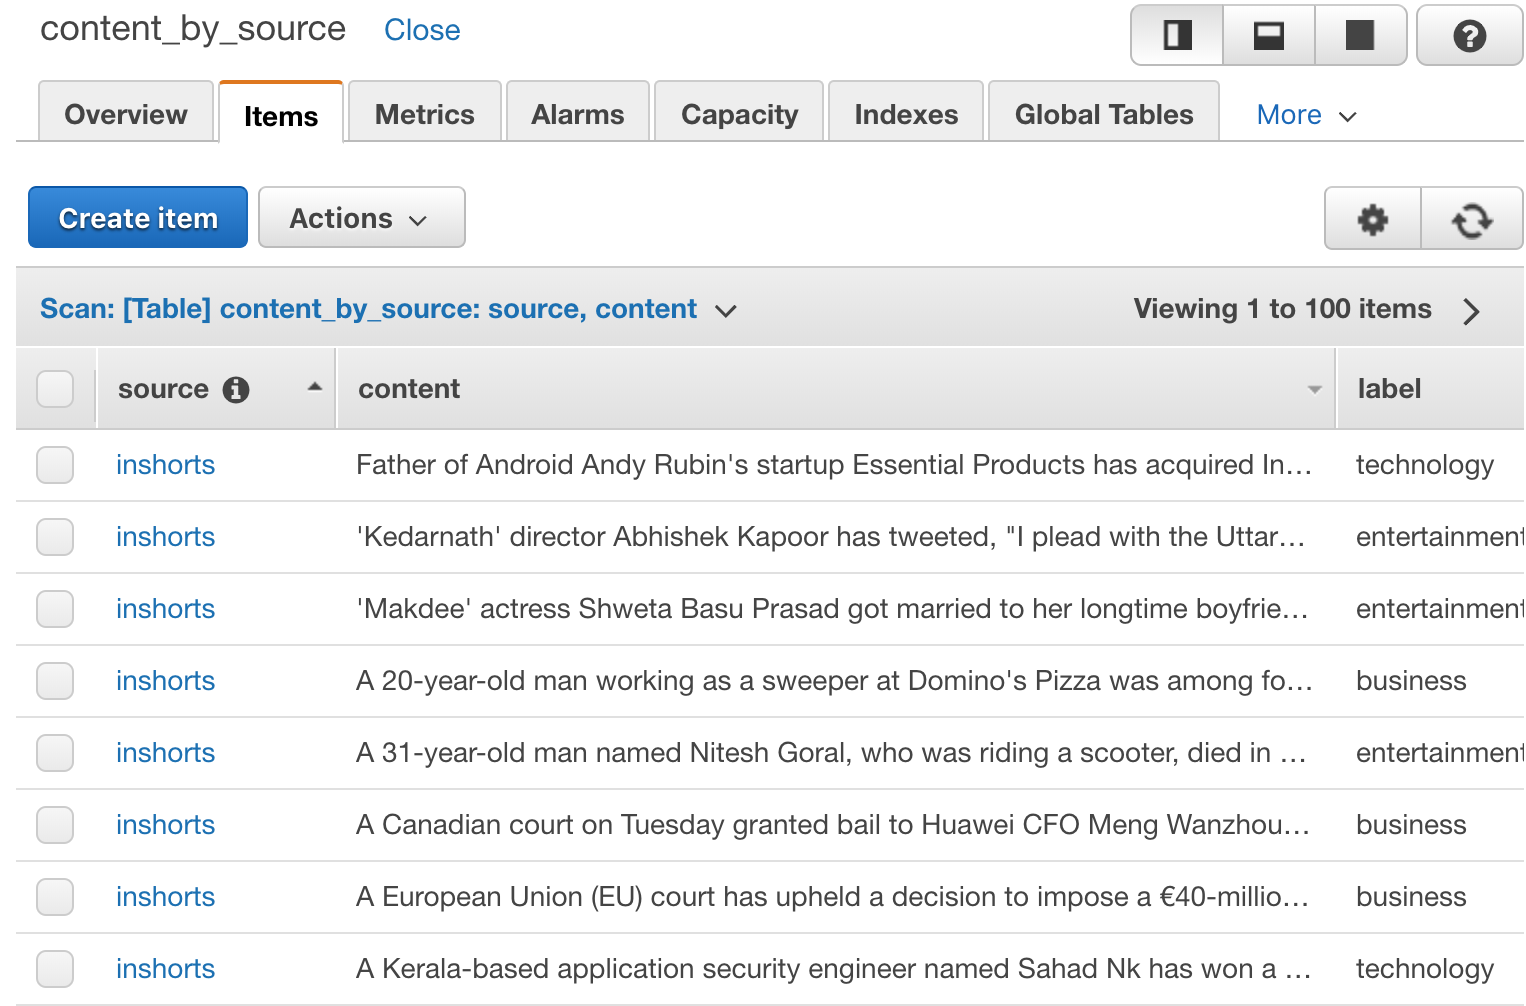
\includegraphics[width=10cm]{dynamo_by_source.png}
    \caption{Fragment tabeli content\_by\_source widocznej z poziomu konsoli AWS}
\end{figure}

\newpage
\section{Warstwa logiki aplikacji}

Elementem centralnym systemu kategoryzacji jest aplikacja komunikująca się z bazą danych używając AWS SDK oraz z warstwą prezentacji danych używając protokołu HTTP. Została ona napisana w języku Python przy użyciu frameworku Flask. Aplikacja jest napisana z wykorzystaniem paradygmatu programowania obiektowego oraz ma budowę komponentową.

\subsection{Python}

Wybór języka programowania zawsze jest pewnym wyzwaniem dla architektów systemu. W tej pracy zdecydowałem się użyć języka Python z następujących powodów:

\begin{enumerate}
    \item Dynamiczne typowanie
    
    Ta cecha języka pozwala nam na bardziej produktywne pisanie pisanie kodu aplikacji. Dynamiczne typowanie zazwyczaj wymaga mniej kodu do wykonania poszczególnych operacji niż statycznie typowane języki. Niestety często skutkuje ona większą podatnością na błędy podczas działania aplikacji.
    
    \item Narzędzia do uczenia maszynowego oraz przetwarzania danych
    
    Popularność języka Python wśród profesjonalistów zajmujących się uczeniem maszynowym oraz analizą danych przyczyniła się do szybkiego rozwoju solidnych narzędzi przystosowanych do tych celów. Pakiety takie jak pandas \footnote{https://pandas.pydata.org/}, tensorflow \footnote{https://www.tensorflow.org}, czy scikit-learn \footnote{https://scikit-learn.org/stable/} znacznie ułatwiają pracę z danymi oraz przyczyniają się do ciągłego rozwoju języka w tym kierunku.
    
    \item Rosnąca popularność
    
    Według raportów portalu Stack Overflow (Rys. \ref{fig:python_popularity}) od roku 2012 ilość pytań zadawanych dla języka Python ma stale tendencję rosnącą, a w ostatnich miesiącach była większa niż dwa kolejne najpopularniejsze języki - Java oraz Javascript. To oznacza stale rosnącą społeczność skupioną wokół tego języka, co znacznie usprawnia proces rozwoju technologii.
    
    \begin{figure}[H]
        \centering
        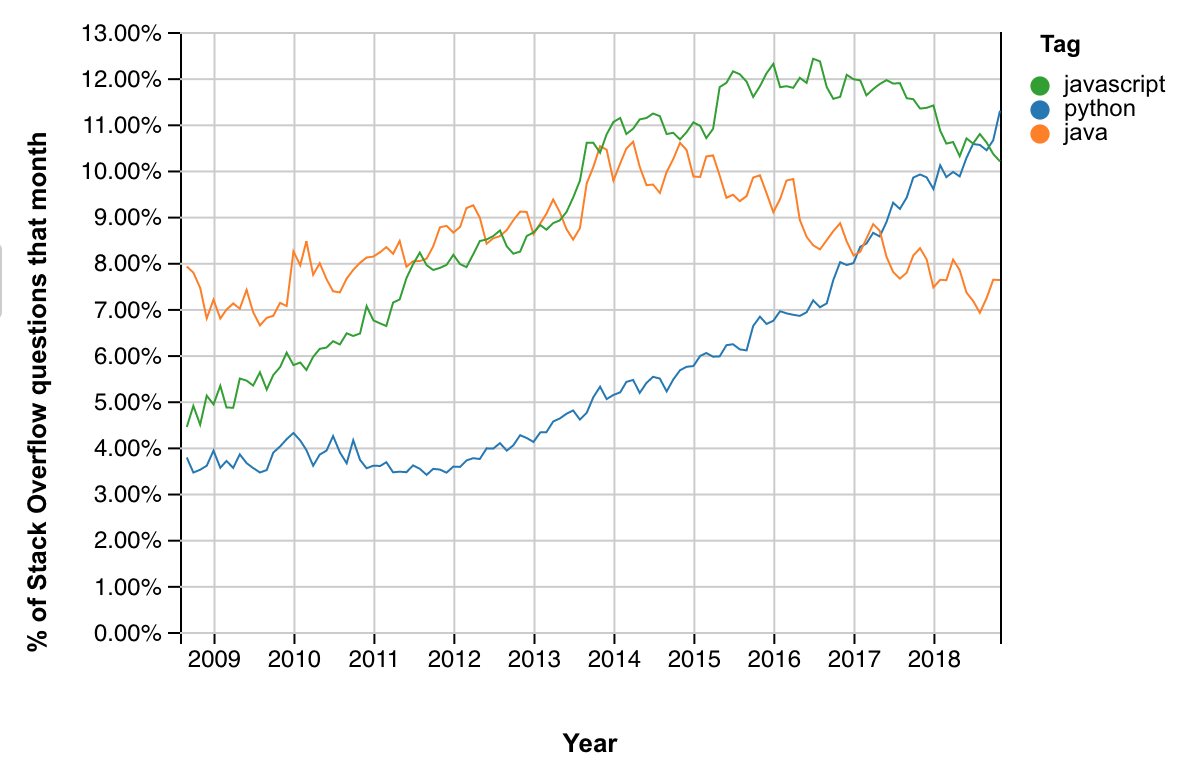
\includegraphics[width=10cm]{python_popularity.png}
        \caption{Popularność pytań o dany język programowania według tagów na Stack Overflow. Źródło: https://insights.stackoverflow.com/trends}
        \label{fig:python_popularity}
    \end{figure}
    
\end{enumerate}

\subsection{Flask framework}

W przeniesieniu logiki na aplikację wykorzystałem projekt Flask \footnote{http://flask.pocoo.org/}. Jest on określany przez autorów jako "microframework" do rozwijania aplikacji webowych. Charakteryzuj go niski próg wejścia - napisanie aplikacji typu "Hello world" to zaledwie 5 linii kodu:

\begin{lstlisting}[language=Python]
from flask import Flask
app = Flask(__name__)

@app.route("/greeting")
def hello():
    return "Hello Flask!"
\end{lstlisting}

W systemie kategoryzacji Flask zapewnił wszystkie funkcjonalności w ramach serwera HTTP, dzięki czemu po jego wdrożeniu będą one dostępne z każdego urządzenia podłączonego do internetu.

\subsection{Architektura}

Z aplikacji można wydzielić dwa główne moduły:
\begin{enumerate}
    \item Moduł danych.
    
    Moduł odpowiadający za gromadzenie, zapis, odczyt oraz migrację danych. Jego podstawowym zadaniem jest pobieranie danych z internetu, przetworzeniu ich do formy możliwej do zapisu (również parsowanie HTML) oraz zapis do bazy danych.
    
    \item Moduł analizy i klasyfikacji.
    
    Pobiera on przygotowane już dane z bazy danych i wykorzystuje je do analizy. Ma również możliwość pobrania wejścia od użytkownika i wykorzystania algorytmów uczenia maszynowego do klasyfikacji wejściowego tekstu.
\end{enumerate}

Każdy moduł jest stworzony zgodnie z paradygmatem programowania obiektowego. Jest on podzielony na klasy, które zostały zaprojektowane zgodnie z zasadami SOLID \footnote{https://pl.wikipedia.org/wiki/SOLID_(programowanie_obiektowe)}

\subsection{Komunikacja z użyciem protokołu HTTP}

Z aplikacją można się komunikować używając protokołu HTTP. Poniżej podane są przykładowe zapytania, których możemy użyć. Pierwsza część określa metodę zapytania, a druga adres URL oraz parametry.

Pobranie danych ze wskazanego źródła:
\begin{verbatim}
    GET {{host}}/data/download?source={{source}}&count={{count}}
    
    {{host}} - adres pod jakim działa aplikacja
    {{source}} - źródło z jakiego chcemy pobrać dane (nazwa API)
    {{count}} - ilość danych jaką chcemy pobrać
\end{verbatim}

Pobranie danych ze wskazanego źródła oraz zmigrowanie ich do bazy danych:
\begin{verbatim}
    POST {{host}}/data/migration?source={{source}}&count={{count}}
\end{verbatim}

Kategoryzacja danych wejściowych na podstawie zmigrowanych danych:
\begin{verbatim}
    GET {{host}}/classify?size={{dataset_size}}&q={{input}}&model={{model}}
    
    {{dataset_size}} - rozmiar zestawu uczącego jaki chcemy użyć
    {{model}} - algorytm uczenia maszynowego za pomocą którego chcemy 
    wykonać klasyfikację
    {{input}} - dane wejściowe dla których wykonujemy kategoryzacją
\end{verbatim}

\newpage
\section{Warstwa prezentacji}

Interfejs użytkownika jest nieodłącznym elementem każdego kompletnego systemu komputerowego. Forma przedstawienia funkcjonalności naszego systemu jest bardzo ważnym aspektem, którego zaniedbanie może zniechęcić użytkowników do korzystania z naszego rozwiązania. Obecnie dużą popularnością cieszą się aplikacje webowe. Są one zbudowane na podstawie dobrze znanych technologii, oraz co najważniejsze - można je otworzyć na wszystkich urządzeniach z zainstalowaną przeglądarką internetową. Spowodowały one częściowe wyparcie technologii desktopowych, które wymagały instalacji oprogramowania na urządzeniu klienta przed jego otworzeniem. Obserwuje się również trend porzucania aplikacji mobilnych na rzecz webowych przystosowanych do telefonów i tabletów.

Z racji popularności technologii HTML, CSS oraz Javascript przeglądarki internetowe stają się coraz bardziej rozbudowanymi narzędziami. Wszystkie popularne przeglądarki udostępniają narzędzia do tworzenia dodatków do nich, a niektóre (np. Google Chrome) oferują możliwość tworzenia aplikacji desktopowych opartych na przeglądarce. Istnieją również projekty jak Electron \footnote{https://electronjs.org/}, które umożliwiają bezpośrednie przekonwertowanie kodu strony internetowej na aplikację uruchamianą bez udziału przeglądarki.

\subsection{Wybór technologii}

Jako warstwę prezentacji do budowanego systemu zdecydowałem się użyć dodatku do przeglądarki Google Chrome. W przypadku systemu kategoryzacji tekstu zaważyły o tym następujące czynniki:
\begin{enumerate}
    \item Możliwość interakcji ze wszystkimi stronami internetowymi.
    
    Internet jest bardzo bogatym źródłem danych w formie tekstu. Poprzez dodatek do przeglądarki użytkownik będzie miał możliwość interakcji z danymi zawartymi w serwisach internetowych i ich analizę i klasyfikację z wykorzystaniem serwisu rozwijanego w ramach tej pracy.
    
    \item Wykorzystanie technologii webowych.
    
    Dodatki do przeglądarek są implementowane w językach używanych do budowy aplikacji webowych. Oznacza to niski próg wejścia - każdy kto miał styczność z językiem Javascript powinien poradzić sobie z ich tworzeniem. Dodatkowo przeniesienie kodu takiej aplikacji do przeglądarki lub na desktop nie będzie wymagało przepisania jej w całości.
\end{enumerate}

Platforma na którą planowałem wdrożyć rozwiązanie to Google Chrome. Według danych NetMarketShare \footnote{https://netmarketshare.com/browser-market-share.aspx} z roku 2018 jest to obecnie najpopularniejsza przeglądarka internetowa:

\begin{figure}[H]
    \centering
    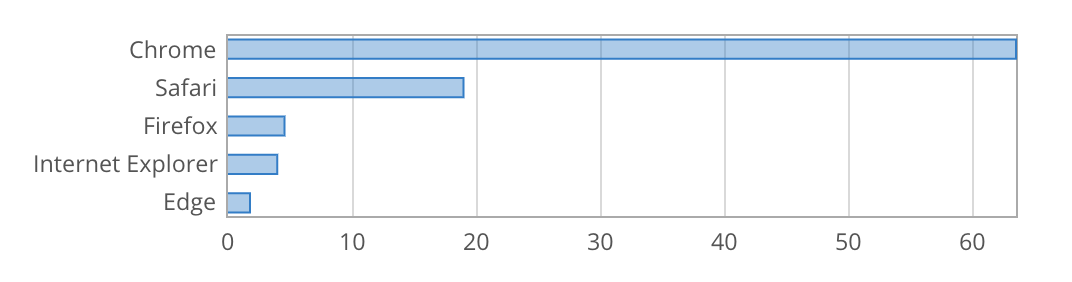
\includegraphics[width=10cm]{browser_market_share.png}
    \caption{Udział przeglądarek w rynku wyrażony w punktach procentowych według NetMarketShare }
\end{figure}

\subsection{Implementacja}

Sercem kodu zawierającego dodatek do przeglądari Google Chrome jest plik manifest.json - dla tej pracy wygląda on tak jak poniżej:

\begin{lstlisting}[language=json]
{
  "manifest_version": 2,
  "name": "Text Recognizer",
  "description": "Extension for recognizing text.",
  "version": "0.1",
  "permissions": [
    "tabs",
    "contextMenus",
    "<all_urls>",
    "storage"
  ],
  "browser_action": {
    "default_popup": "popup.html",
    "default_title": "Text Recognizer"
  },
  "content_scripts": [
    {
      "matches": [
        "<all_urls>"
      ],
      "js": [
        "selection.js"
      ],
      "run_at": "document_start",
      "all_frames": true
    }
  ],
  "background": {
    "scripts": ["background.js"]
  },
  "options_ui": {
    "page": "options.html",
    "open_in_tab": false
  }
}
\end{lstlisting}

Poza definicjami wyświetlanych tytułów oraz wersjonowania zawiera on najważniejsze informacje o pozwoleniach na akcje oraz dostęp do poszczególnych elementów przeglądarki. Pozostałe sekcje obejmują informacje o strukturze dodatku: 

\begin{enumerate}
    \item Browser action
    
    Definiuje tytuł oraz ścieżkę do elementu typu pop-up, który pojawia się w momencie kliknięcia na ikonę dodatku.
    
    \begin{figure}[H]
    \centering
    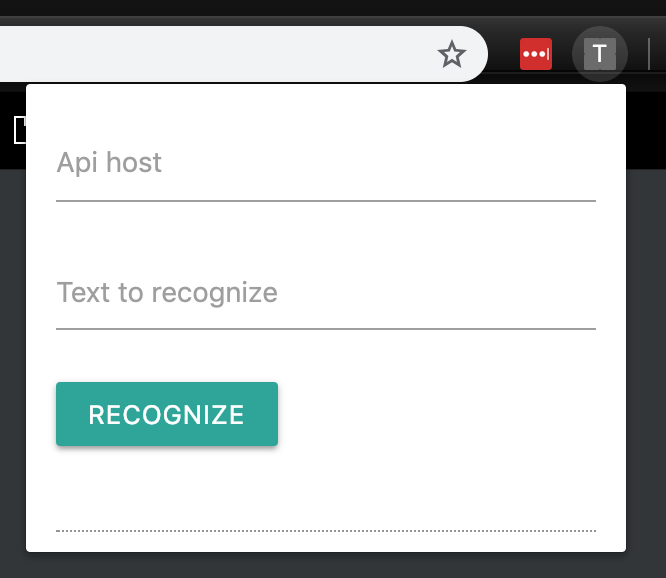
\includegraphics[width=10cm]{images/implementacja/popup.png}
    \caption{Popup}
    \end{figure}
    
    \item Content scripts
    
    Problem związanym ze wspomnianym wcześniej elementem zdefiniowanym jako browser action jest posiadanie osobnego elementu DOM (Document Object Model\footnote{https://www.w3.org/TR/DOM-Level-2-HTML/}). Poprzez sam popup nie mamy możliwości jakiejkolwiek interakcji z obecnie otworzoną stroną internetową. Rozwiązaniem jest użycie content script, który jest uruchamiany w kontekście strony. Ma on możliwość interakcji z modelem DOM oraz komunikacji z elementem popup poprzez system wiadomości. W mojej aplikacji content script służy do przesłania zaznaczonego tekstu do elementu popup, jeśli dostanie takie żądanie w wiadomości. Jego kod wygląda tak jak poniżej:
    
    \begin{lstlisting}[language=javascript]
    chrome.extension.onMessage.addListener((request, sender, sendResponse) => {
    if (request.method == "getSelection")
        sendResponse({data: window.getSelection().toString()});
    else
        sendResponse({data: ''});
    });
    \end{lstlisting}
    
    \item Background
    
    Skrypty zdefiniowane w sekcji background działają w tle strony niezależnie od jej zawartości. Wykorzystuję go do ustawienia nowego elementu w menu kontekstowym, ustawienia funkcji 'onclick' oraz przekazanie do niej obecnie zaznaczonego tekstu.
    
    \begin{figure}[H]
    \centering
    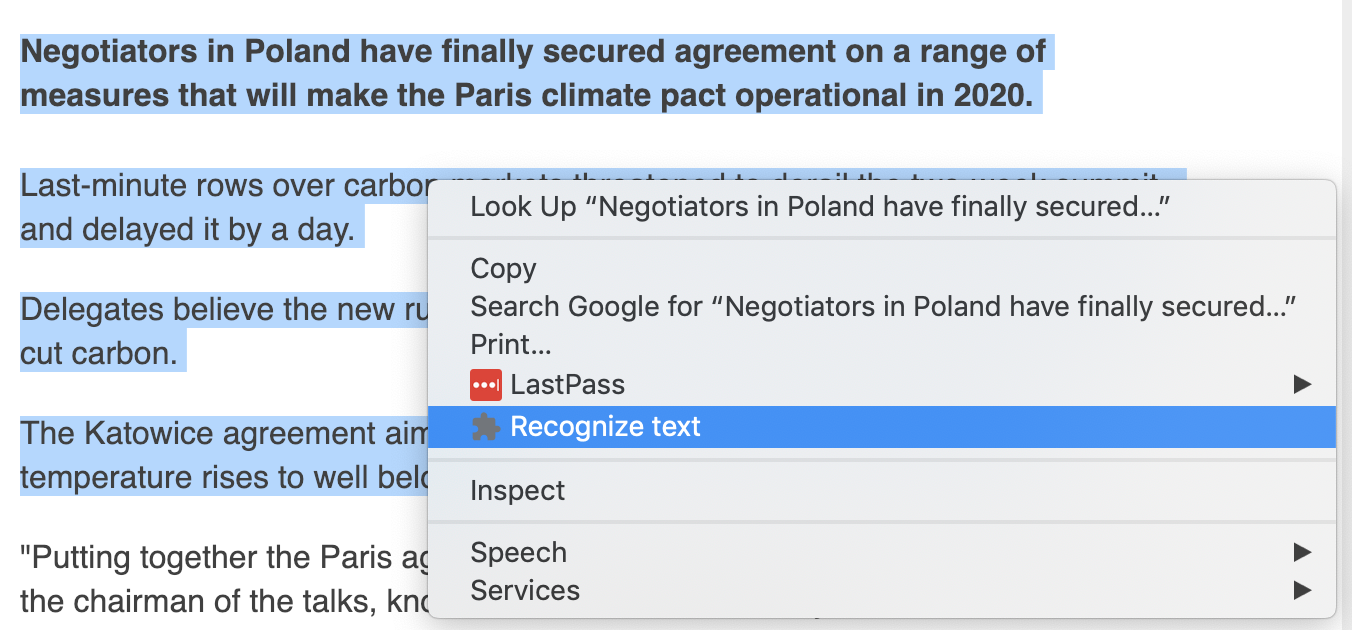
\includegraphics[width=10cm]{images/implementacja/context_menu.png}
    \caption{Menu kontekstowe}
    \end{figure}
    
    \item Options UI
    
    Definiuje stronę z ustawieniami dodatku. Do przechowywania konfiguracji w przeglądarce możemy użyć obiektu 'storage' dedykowanego dla dodatków przeglądarki Chrome - przed użyciem musimy umieścić go w liście 'permissions' pliku manifest. 
    
    \begin{figure}[H]
    \centering
    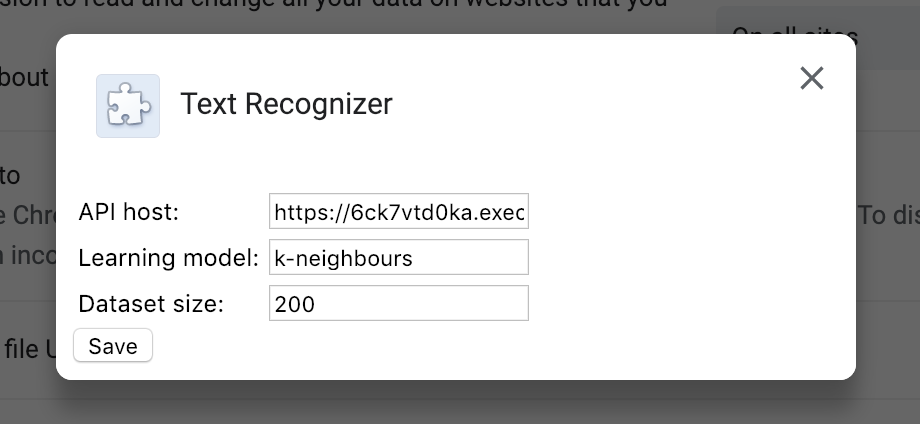
\includegraphics[width=10cm]{images/implementacja/options.png}
    \caption{Panel ustawień}
    \end{figure}
    
\newpage
\section{Architektura}

Wysokopoziomową budowę systemu można przedstawić za pomocą diagramu \ref{fig:architecture}. Warstwę prezentacji, za pomocą której użytkownik komunikuje się z systemem jest dodatek do przeglądarki Chrome. On natomiast używa zapytań HTTP do wymiany informacji z warstwą logiki aplikacji (Serwis klasyfikacji), której funkcję pełni aplikacja napisana w języku Python. Oprócz odpowiadania na żądania użytkownika ma on jeszcze dwie główne funkcjonalności - pobieranie danych z serwisów internetowych oraz zapisywanie ich oraz odczytywanie z warstwy persystencji danych, której rolę pełni DynamoDB.

    \begin{figure}[H]
    \centering
    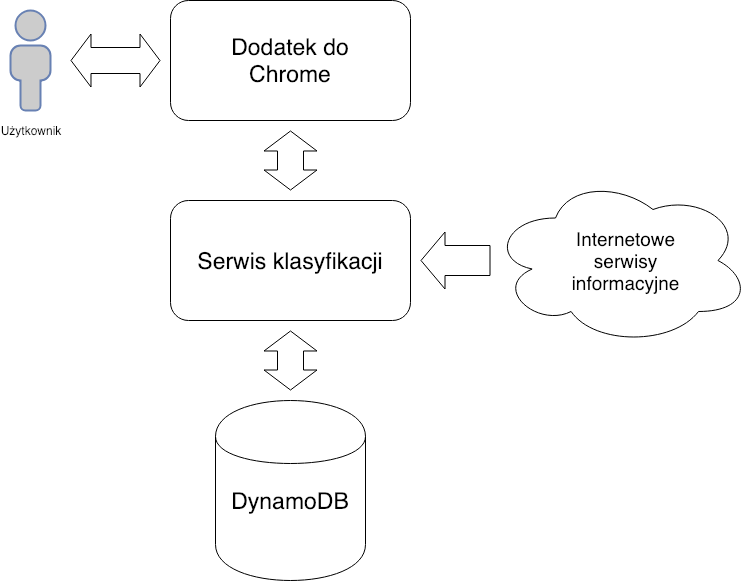
\includegraphics[width=12cm]{images/implementacja/architecture.png}
    \caption{Wysokopoziomowa architektura systemu}
    \label{fig:architecture}
    \end{figure}
    
\end{enumerate}